%!TEX root = ../thesis.tex
\chapter{Conclusion}
\label{chapter_conclusion}

We have presented five authoring systems for creating and following instructions from author demonstration. This final chapter restates the contributions of this dissertation and discusses the synthesis of our tools and future directions.

\section{Restatement of Contributions}
This dissertation has demonstrated video-based computational approaches that support tutorial creation and consumption. A set of interactive systems that generate concise instructions from author demonstrations are introduced. Design and technical contributions of this work can be summarized as follows:

\begin{itemize}
  \item New instructional formats that consider learning factors.
    \begin{itemize}
      \item Mixed-media tutorials composed of step-by-step static instructions and in-place video clips to demonstrate individual operations.
      \item Enhanced video playback that contains dynamic glyphs to provide viewers awareness to the upcoming input event.
    \end{itemize}
  \item Authoring workflows in an easy-to-setup environment for amateur users to create effective instructions by demonstration.
    \begin{itemize}
      \item Methods and user interfaces for recording, reviewing, and editing an instructional task with the support of software and capturing devices.
      \item Multi-modal interfaces using motion and voice commands or touch interaction to author step-by-step instructions while performing physical demonstrations.
    \end{itemize}
  \item Automatic or semi-automatic approaches using video and audio analysis that includes users in the loop to produce high-quality results.
    \begin{itemize}
      \item Algorithms of analyzing video, audio, and motion data using computer vision and signal processing approaches to segment a demonstration.
      \item Techniques for combining high-level user annotations with content analysis to generate concise instructions.
    \end{itemize}
\end{itemize}

% How to design tutorial systems appropriately for different situations
% * level of expertise of instructor, learner
% * what are you trying to make easier?

\section{Future Directions} %Remaining Challenges and

Our tools provided evidence how computer technologies could assist amateur authors in creating instructional content, which in turns enhance the learning experiences. Based on these design experiences, we propose directions of future research in computational instruction design.

\subsection{Beyond a Single User and Linear Instructions}
The authoring systems presented in this dissertation mainly focus on supports of a single user in a software domain (i.e., MixT and DemoWiz that capture one software application walk-through) or physical tasks (including DemoDraw that records an author's movements).
%
The DemoCut system analyzes one single, static video shot. The example videos we tested included only one demonstrator. We argue that our techniques can possibly apply for content that contains multiple demonstrators' activities and narrations, but our authoring interfaces are designed for a single author.
%
Finally, the Kinectograph recording device supports two demonstrators in a scene, and the tablet interface can be possibly controlled by both users at the same time.

\subsubTitleBold{Tool Support for a Team}
We acknowledge the need of expanding our designs to support multiple users. From the authoring perspective, a demonstration can include several demonstrators~\tofix{citation here}. For examples, cooking and assembly tasks (e.g., for furniture or larger machines) are commonly collaboratively achieved by two or more people. Demonstrators may have different roles, such as one as the main instructor, wile the other(s) serve as supporters or a learner. For another example, dancers may have different moves in a choreography.
%
Researchers have proposed methods of detecting activities of multiple people in a video~\tofix{citation here} and video editing~\tofix{Amy's UIST'16 work here}, but authoring instructions collaboratively is still an open topic. In addition, professional filmmaking is commonly by teamwork, where a group of people forms a production team and contributes in different stages, including planning, shooting, and editing~\tofix{citation here}. We see research opportunities in supporting large projects or complicated activities that involve long time (e.g., a few days to weeks) and collaborators (e.g., a director records a demonstrator's making process.)

\subsubTitleBold{Tool Support for Human-Robot Collaboration}
feedback for physical authoring~\cite{Agrawal:2015:PPS:2807442.2807505,Zoran:2013:FFD:2470654.2481361}, HRI construction~\cite{Vasey:2016:HHR:2897839.2927404}

\subsubTitleBold{Tool Support for Alternatives}
sharing - iterative, branching

\subsection{Understanding of Expertise}

\subsection{Learning from Instructions}

software learnability~\cite{Grossman:2009:SSL:1518701.1518803}
formal language
- now template, a set of techniques
machine learning

\subsection{New Sensing Techniques}
Tango, Structure Sensor, Leap Motion

hand tracking~\cite{taylor-siggraph2016}
Fusion4D~\cite{dou-siggraph2016}

\subsection{Emerging Instructional Space}

Augmented and virtual reality systems are becoming available to end users via affordable forms. However, designing AR and VR experiences extremely requires expertise and efforts. As devices offer personalized effects supported by sensing and input techniques, we need new authoring tools that focus on delivering story-centric experiences. Tools should also enable both professionals and amateurs to create and iterate designs efficiently in an immersive 3D world. ...research what future AR and VR creation tools would look like with new authoring processes.

~\cite{MicrosoftHoloLensSkype,Gurevich:2012ko}

by demonstration~\cite{MotionBuilderAR}

\begin{figure*}[ht!]
  \centering
  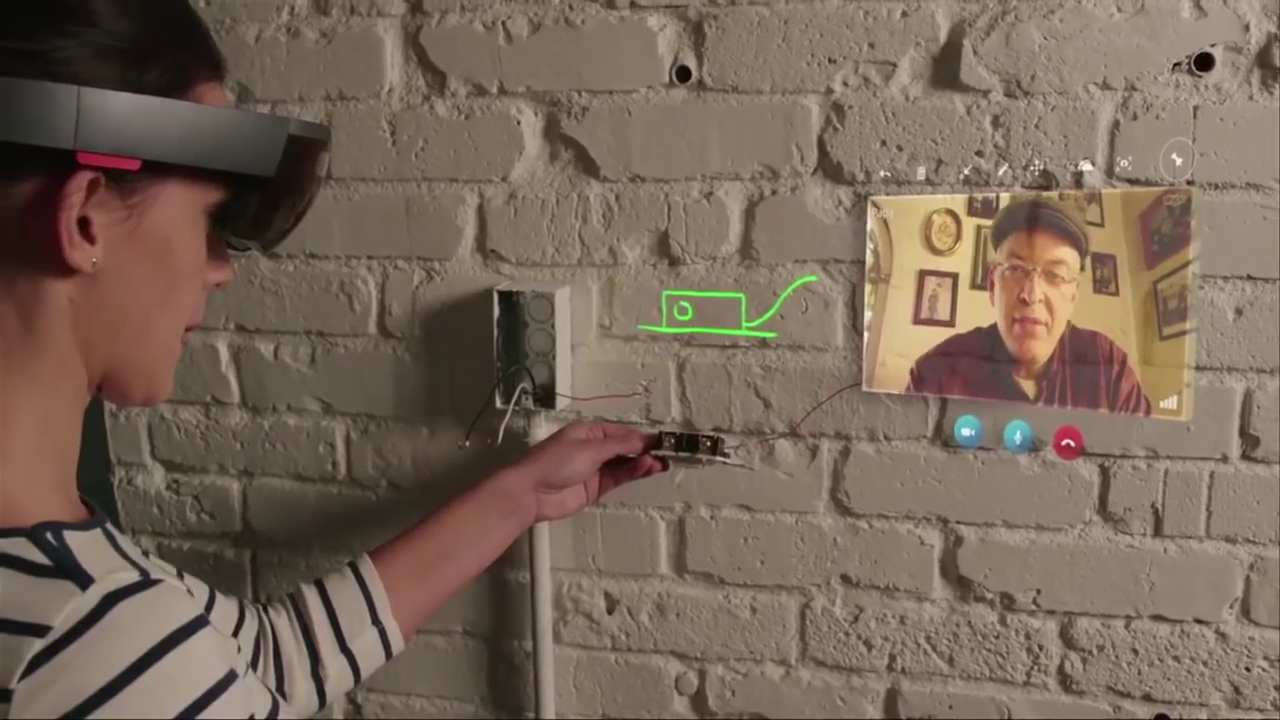
\includegraphics[width=0.4\textwidth]{\conclusion/fig/ar/hololens_fix1}
  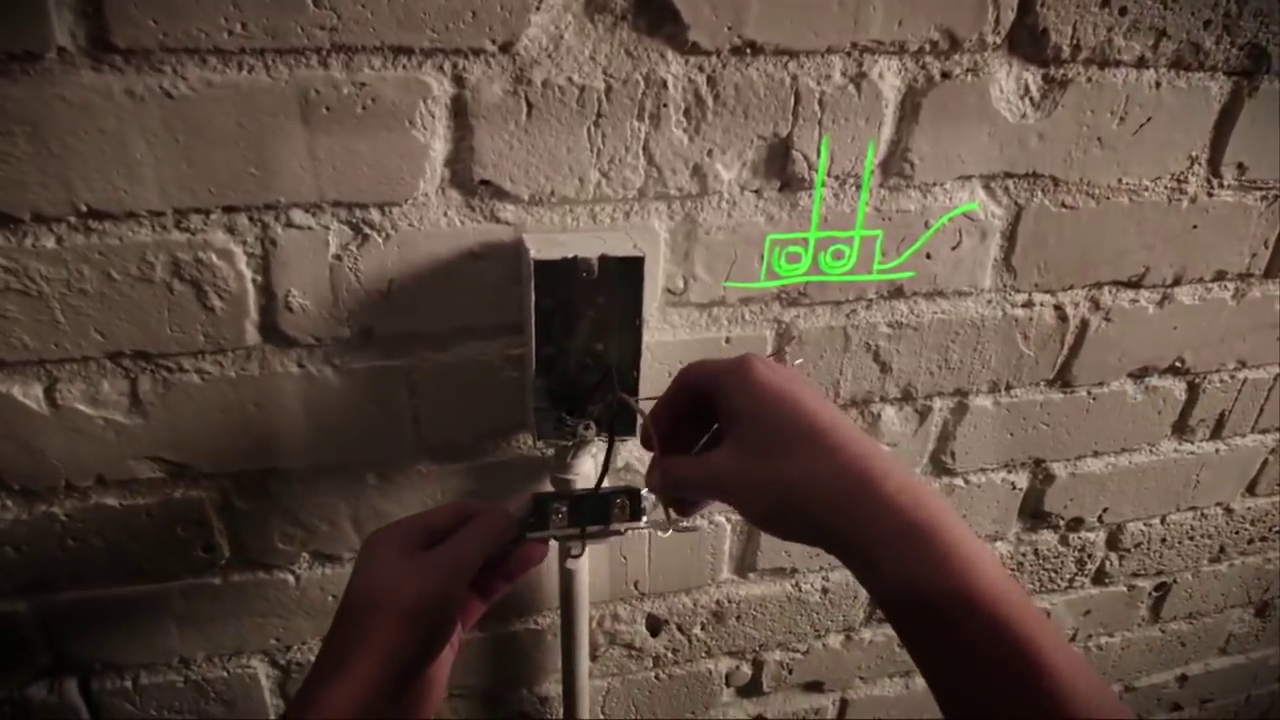
\includegraphics[width=0.4\textwidth]{\conclusion/fig/ar/hololens_fix2}
% \begin{tabular}{cc}
%   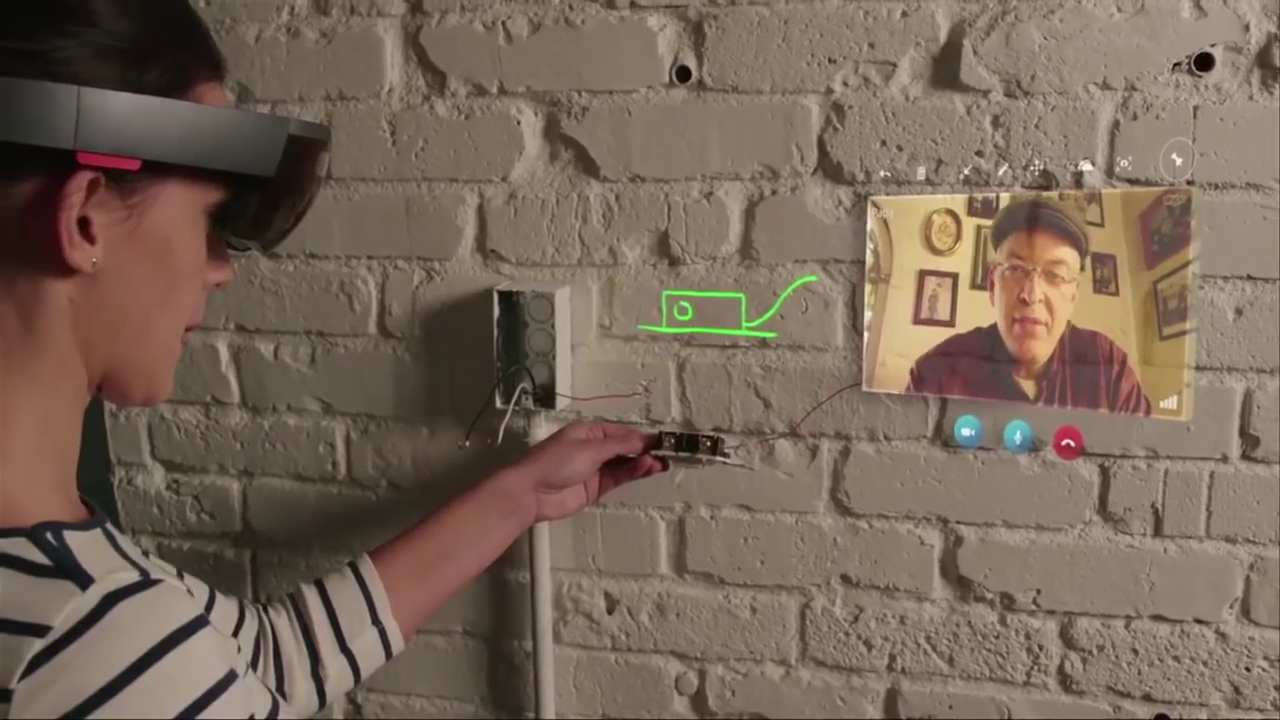
\includegraphics[width=0.4\textwidth]{\conclusion/fig/ar/hololens_fix1} &
%   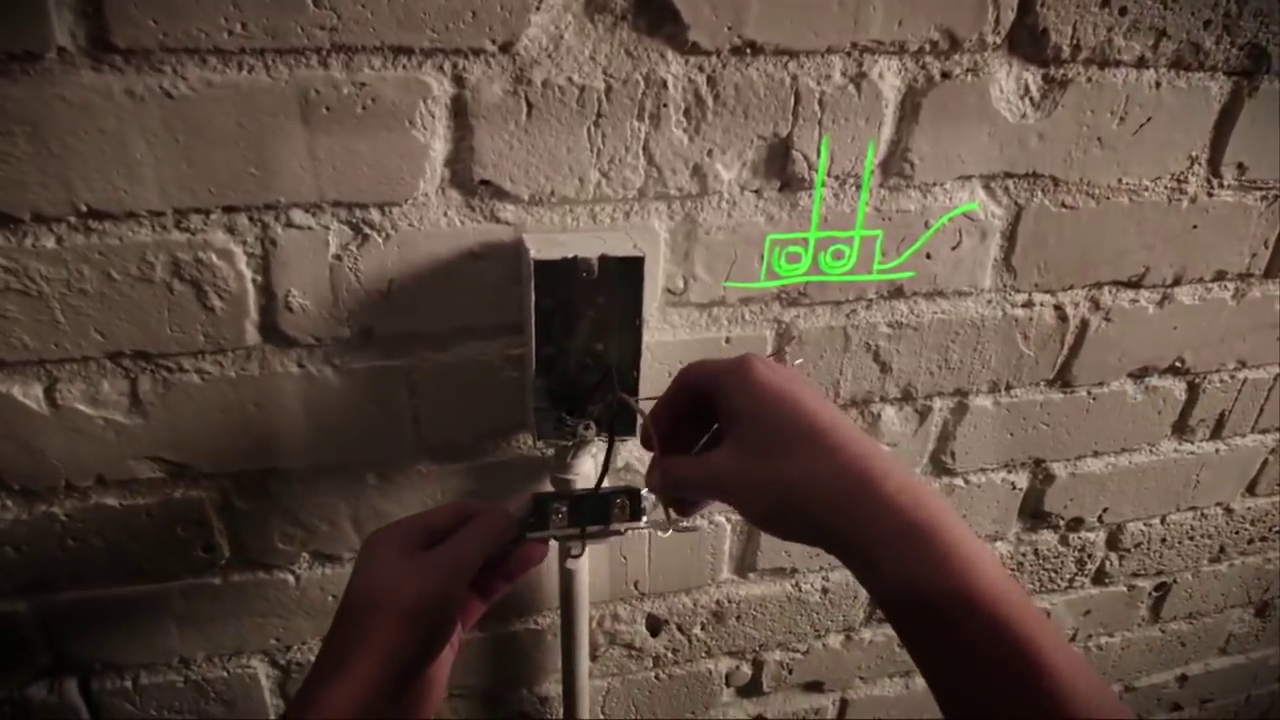
\includegraphics[width=0.4\textwidth]{\conclusion/fig/ar/hololens_fix2} \\
% \multicolumn{2}{c}{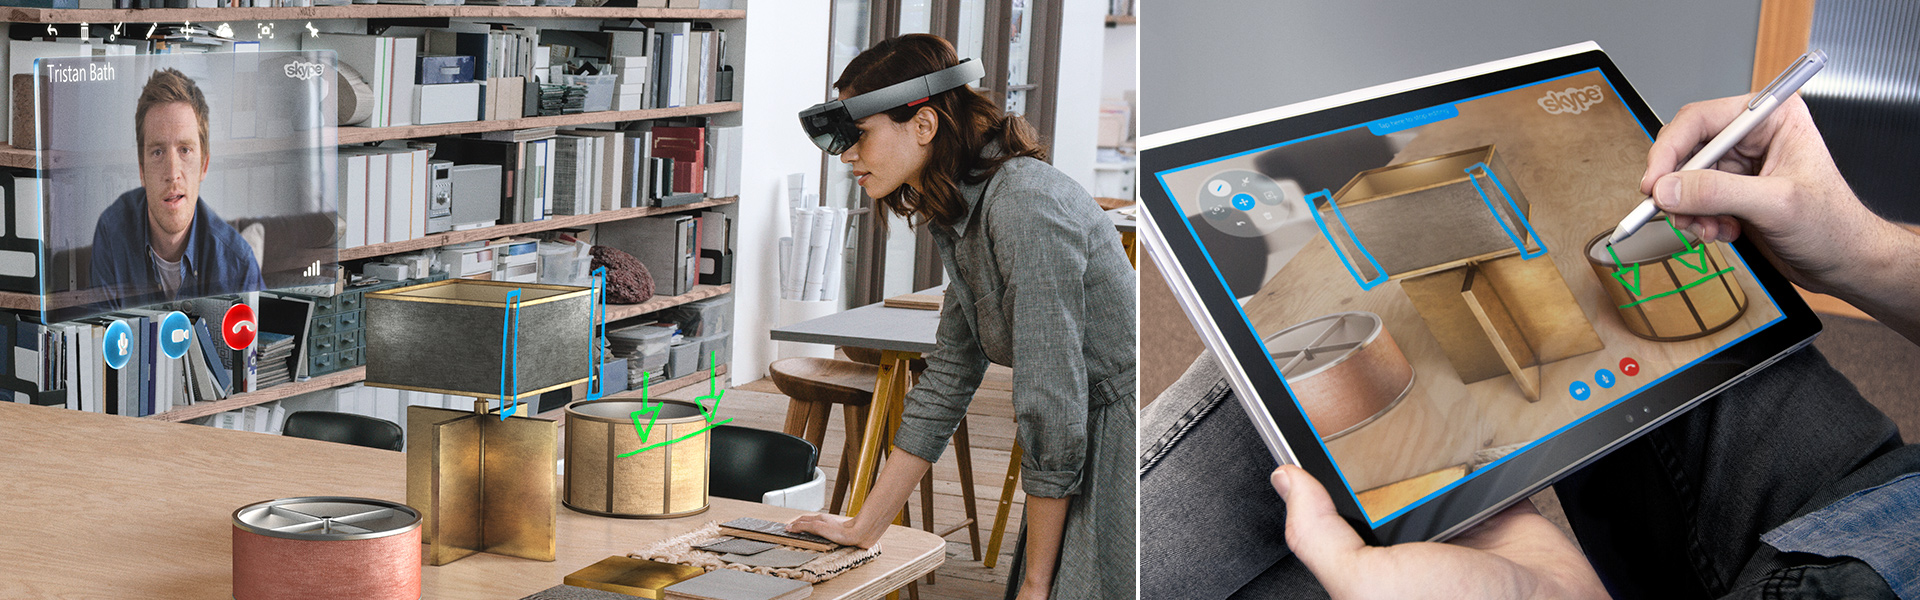
\includegraphics[width=0.82\textwidth]{\conclusion/fig/ar/hololens_skype} }
% \end{tabular}
\caption{
  Recent Augmented Reality (AR) applications have demonstrated ways of providing real-time physical instructions from a remote instructor~\cite{MicrosoftHoloLensSkype,Gurevich:2012ko} or enhancing desktop editing, such as reviewing character animation shown in this figure~\cite{MotionBuilderAR}, licensed under CC BY 2.0.
}
\end{figure*}

VR: capture physical instructions and share with others
authoring tools for immersive experiences

\section{Summary}
In this dissertation, we present video-based approaches designed for amateur users to produce and consume effective instructions from demonstrations. Using video and audio analysis techniques, our tools support recording, editing, and playback in a tutorial production process. We demonstrate results of a set of five computer-generated tutorials we designed for several instructional domains, including software applications and physical activities. Our results increase the quality of instructions created by tutorial authors and support learners navigating and following the tutorials.
